%%%%%ADD IN TRACKER RESOLUTION
\section{Tracking System}
The tracker is CMS's inner-most detector. The purpose of the 
tracker is to reconstruct the trajectories of charged particles 
coming from the LHC collisions and measure the charged particle momenta. 
These charged particles leave a path in the tracker material referred to as a 'track'. %fix
These tracks are then used in the reconstruction of electrons, muons, taus, hadrons and jets 
and are also used to determine the primary vertex of an interaction. Additionally, 
the tracker can be used in the identification of displaced vertices which are located
away from the primary vertex; a displaced vertex (or 'secondary vertex') is 
a decay signature that is often present 
in heavy (b or c -flavored) jets.
As can be seen in Figure \ref{fig:trackerLayout}, the CMS tracker consists of two main 
detectors: an inner silicon pixel detector and an outer silicon strip detector. 
\begin{figure}[hb]
  \centering
	\includegraphics[width=1\textwidth]{trackerImages/trackerLayout.png}
  	\caption[CMS Tracker Layout]
   	{CMS Tracker layout}
	\label{fig:trackerLayout}
\end{figure}
Efficient reconstruction of collisions require a low hit occupancy, a high hit redundancy and a
fast response such that tracks can be identified reliably and attributed to the correct bunch crossing.
Low hit occupancy can be achieved with high granularity while high hit redundancy requires
many detector layers. These former two requirements are only achieved with a 
high power density of on detector electronics which require efficient cooling. 
Unfortunately, this directly conflicts with the goal to limit the material 
budget of the tracker; interaction with material results in Coulomb scattering,
bremsstrahlung, nuclear interactions and photon conversion. Finally, an extremely
high particle flux results in radiation damage to the silicon sensors mainly 
in the form of modifications to the silicon crystal lattice. 
The aforementioned objectives and constraints resulted in a tracker design 
based entirely on silicon detector technology. 
At 5.4 m in length and 2.2 m in diameter, the CMS tracker is the largest inner
silicon detector ever built in a high energy physics experiment.
\begin{figure}[hb]
  \centering
  \begin{subfigure}[b]{.45\textwidth}
	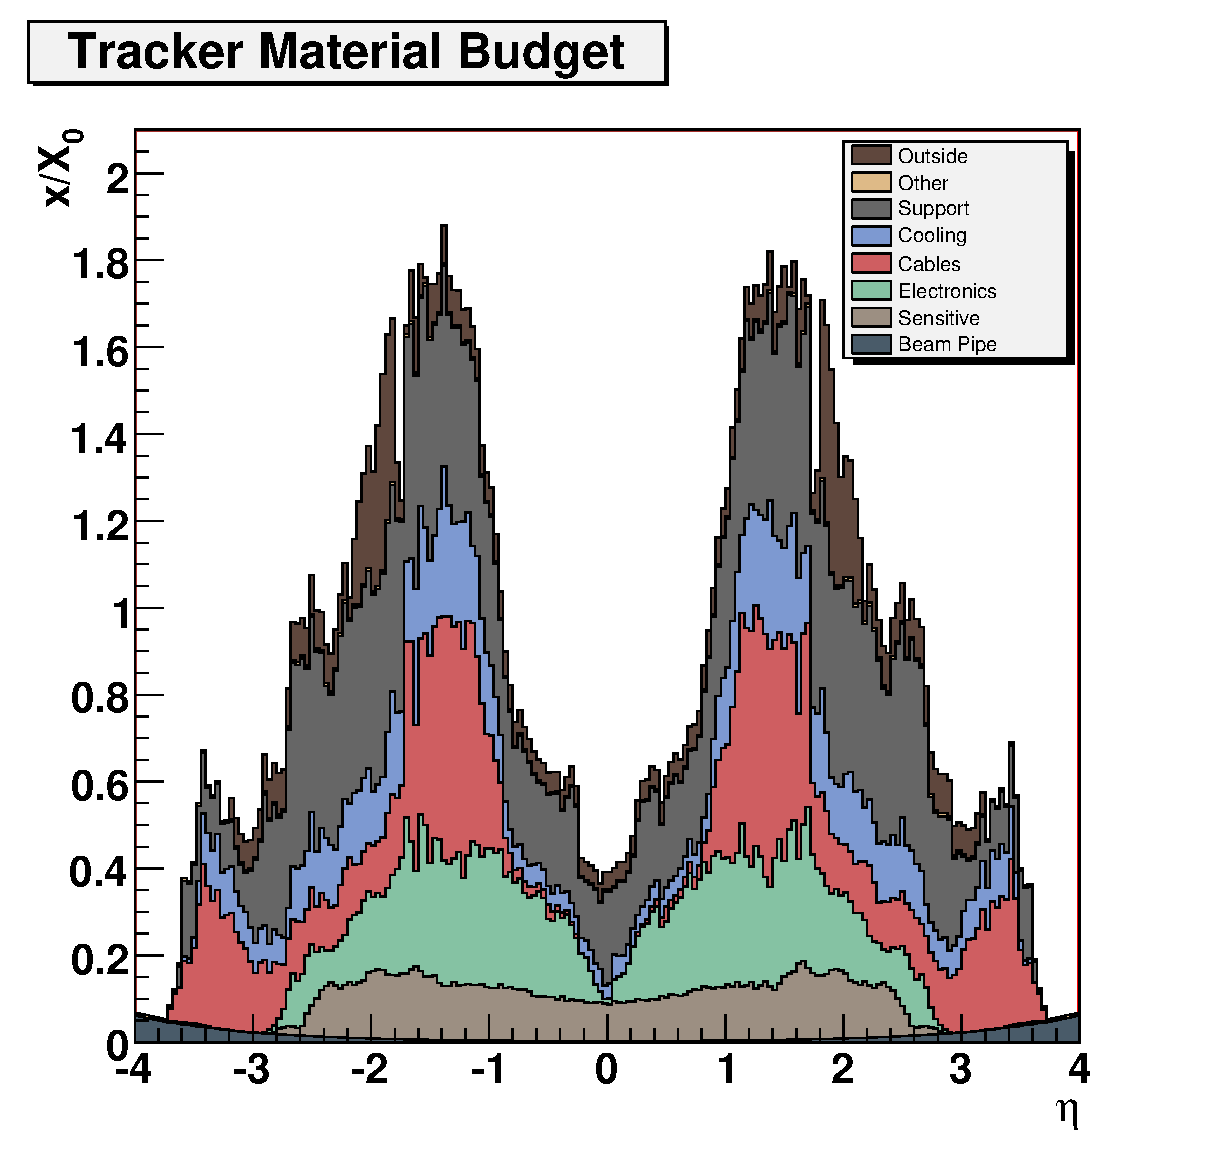
\includegraphics[width=\textwidth]{images/Tracker_Materials_x_vs_eta.eps} 
	\end{subfigure}	
   \begin{subfigure}[b]{.45\textwidth}
	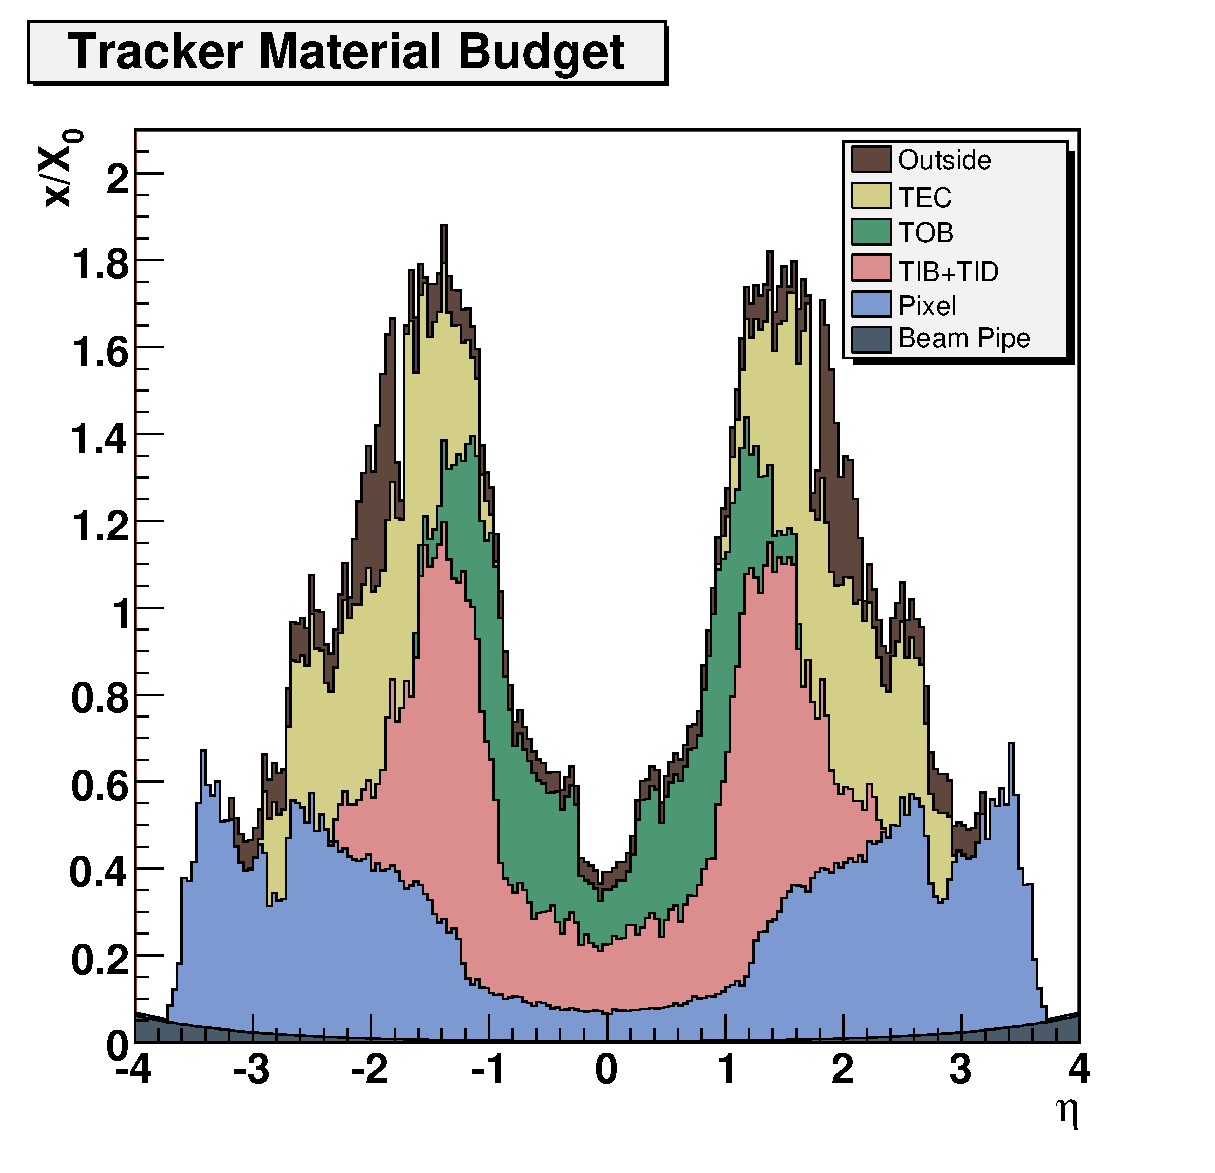
\includegraphics[width=\textwidth]{images/Tracker_SubDetectors_x_vs_eta.eps}
    \end{subfigure}	
  	\caption[Tracker Material Budget]
   	{Tracker material budget, x/$X_{0}$ vs. $\eta$}
	\label{fig:trackerMaterial}
\end{figure}

The material budget of the tracker can be characterized by the rate at which a particle
passing through it loses energy. The radiation length, $X_{0}$, is the 
mean distance over which a high-energy electron loses all but 1/$e$ 
of its energy by bremsstrahlung %citation needed p.291 PDG ------
and $\frac{7}{9}$ of the mean free path for pair production by 
a high-energy photon. Figure \ref{fig:trackerMaterial}
shows the material budget of the CMS tracker in terms of radiation length as a function of $\eta$. 
Due to the location of cabling, electronics and other services, the material budget of the 
tracker is at a minimum of 0.4 $X_{0}$ at $\eta \approx 0$ and increases to approximately 1.8 $X_{0}$
at $|\eta| \approx 1.4$, after which it decreases. 

%Resolution on the order of 10 micro meters http://arxiv.org/pdf/1007.1988.pdf
\subsection{Pixel Detector}%%%check to be sure where you say pixel system vs. pixel detector 
The pixel detector is the inner most detector of the tracking system and,
covering the region from 4 to 15 cm in radius, is the closest detector to 
the interaction point. It has a high granularity and contributes precise 
tracking points in $r-\phi$ and $z$ and is therefore responsible for a small impact 
parameter resolution that is important for b and c-jet secondary
vertex reconstruction and $\tau$-lepton secondary vertex reconstruction.

\begin{figure}[hb]
  \centering
	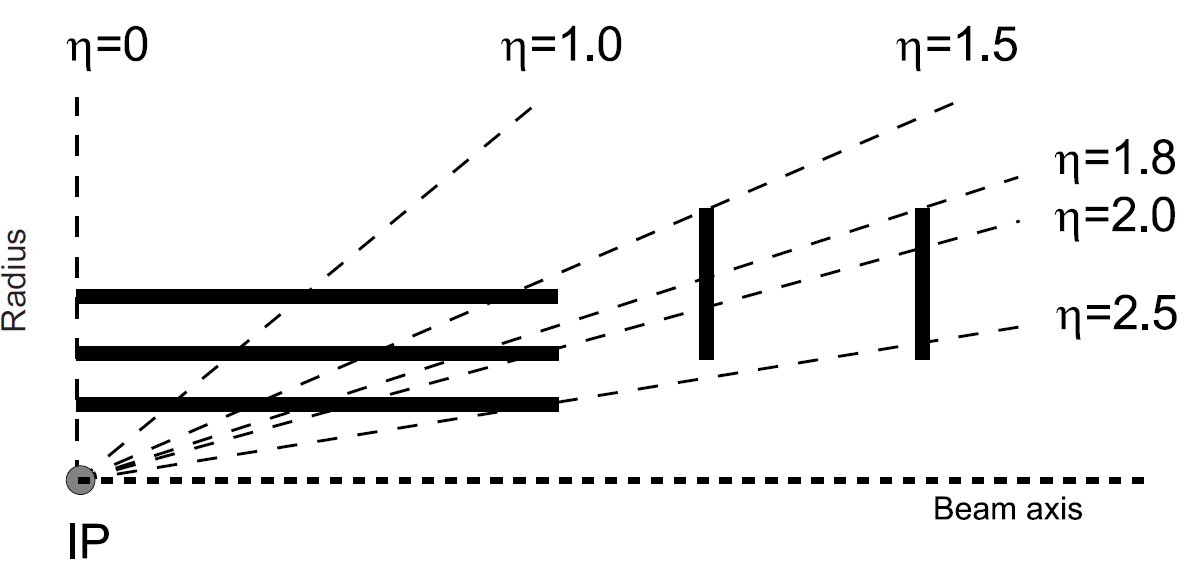
\includegraphics[width=0.7\textwidth]{images/pixelLayout.png}
  	\caption[Pixel System Layout]
   	{Pixel System Layout}
	\label{fig:pixelLayout}
\end{figure}

The pixel detector is made up of individual pixel cells with a size of 
100 $\times$ 150 $\mu m^{2}$; it has 66 million active elements and covers
a surface area of 1 $m^{2}$. The pixel detector is composed of three barrel 
layers and two endcap disks for which the pseudorapidity range from $-2.5<\eta<2.5$.
The three barrel layers are located at mean radii of 4.3, 7.3, and 10.2 cm. 
The endcap disks extend from 4.8 to 14.4 cm in radii are located at a mean distance
of $z=\pm35.5$ cm and $z=\pm48.5$ cm from the interaction point. 
As can be seen in figure \ref{fig:pixelLayout} this arrangement allows for 3 tracking points over 
almost the full $\eta$-range of the pixel system. Due to 
particles entering the detector at an average angle of $20^{\circ}$ 
charge-sharing between pixels is achieved which improves position resolution.

The pixel system has a zero-suppressed read out scheme with analog pulse
height read-out. This improves the position resolution due to charge sharing,
it helps to separate signal and noise hits as well as to identify large hit 
clusters from overlapping tracks.
A position resolution on the order of 10 $\mu m$ is achieved.

\subsection{Silicon Strip Tracker}
The silicon strip detector is located outside the inner pixel detector, 
It extends from 25 cm to 110 cm in radius and pseudorapidity up to $|\eta|<2.5$. 
This region has a particle flux on 
the order of 100 times less than what is seen by the inner most layers of 
the pixel detector. It is a complementary system to the inner pixel
detector and has a lower granularity. The silicon strip detector 
has 9.3 million active elements over a total surface area of 198 m$^{2}$
and consists of 3 large subsystems. As can be seen in figure \ref{fig:trackerLayout}, 
the Tracker Inner Barrel and Disks (TIB/TID) extend in radius to
55cm and are composed of four barrel layers with three disks at each.
The Tracker Outer Barrel (TOB) consists of six barrel layers and extends to $\pm118$ cm
in z. Extending beyond this in the z-direction, the Tracker EndCaps (TEC+ and TEX- where the plus and minus
indicate the direction in z) are located from 124cm $<|z|<$280 cm. They are composed of 
nine disks which are populated with up to seven rings of radial-strip silicon detectors.
The combined layouts of the pixel detector and silicon strip detector
result in 8 to 14 high precision measurements of track impact points for 
$|\eta|<2.4$.

The tracker resolution of muon $p_{T}$ as a function of $p_{T}$ and pseudorapidity are 
shown in figure \ref{fig:TrackerResolution}.
At high momentum (100 GeV), the $p_{T}$ resolution is approximately 2-3\%. The degradation at
$|\eta|\approx 1$ and beyond is due to the gap between barrel and the end-cap disks
and due to inferior hit resolution of the last hits of the track measured in TEC ring 7. 
In the barrel, tracker resolution ranges from $\approx$1-2\% from 1 to 100 GeV while
in the endcap tracker resolution ranges from $\approx$2-7\% from 1 to 100 GeV. High
$p_{T}$ muons benefit from a combined fit between tracks found in the tracker and
 tracks found in the muon system for an improved $p_{T}$ resolution.

\begin{figure}[hb]
\centering
  \begin{subfigure}[b]{.475\textwidth}
	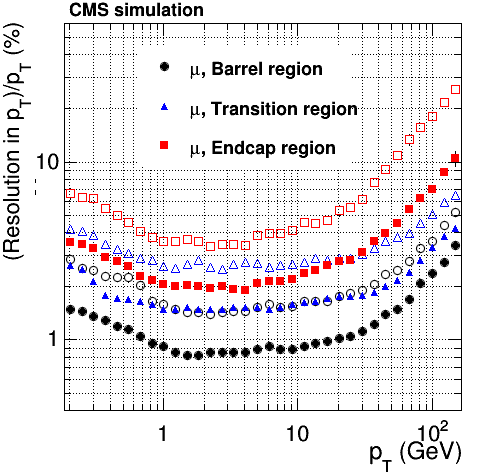
\includegraphics[trim = 0mm 0mm 0mm 0mm, clip,width=\textwidth]{images/resolutionPtVsPt.png}
	\end{subfigure}	
   \begin{subfigure}[b]{.475\textwidth}
	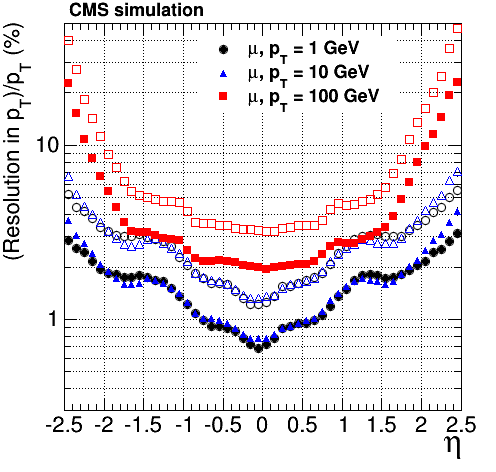
\includegraphics[trim = 0mm 0mm 0mm 0mm, clip,width=\textwidth]{images/resolutionPtVsEta.png}
    \end{subfigure}	
  \caption[]
   	{Tracker $p_{T}$ resolution as a function of $p_{T}$ and $\eta$. The sold (open) markers correspond to the half-widths for the 68\% (90\%) intervals centered on the peak of the distribution \cite{TRK11001}.}
    \label{fig:TrackerResolution}
\end{figure}